% !Mode:: "TeX:UTF-8:Main"

\documentclass{article}
\usepackage{l3pdf,pdfresources}
\ExplSyntaxOn
\pdf_uncompress:
\ExplSyntaxOff

\usepackage{ifluatex,graphicx}
\usepackage{pdfpages}
\usepackage[customdriver=hgeneric-experimental]{hyperref}
%\usepackage{newpax}
%\usepackage{luacode}
%\begin{luacode}
%\usepackage{luatex85}
\ifluatex
\directlua{
 require("newpax.lua")
% print("XXXXXX",newpax.writepax,newpax.writenewpax)
 newpax.writenewpax("pax-input")
% newpax.writepax("pax-input")
 }
\usepackage{newpax}
\else
\usepackage{newpax}
\fi
%\end{luacode}

\begin{document}
blub
%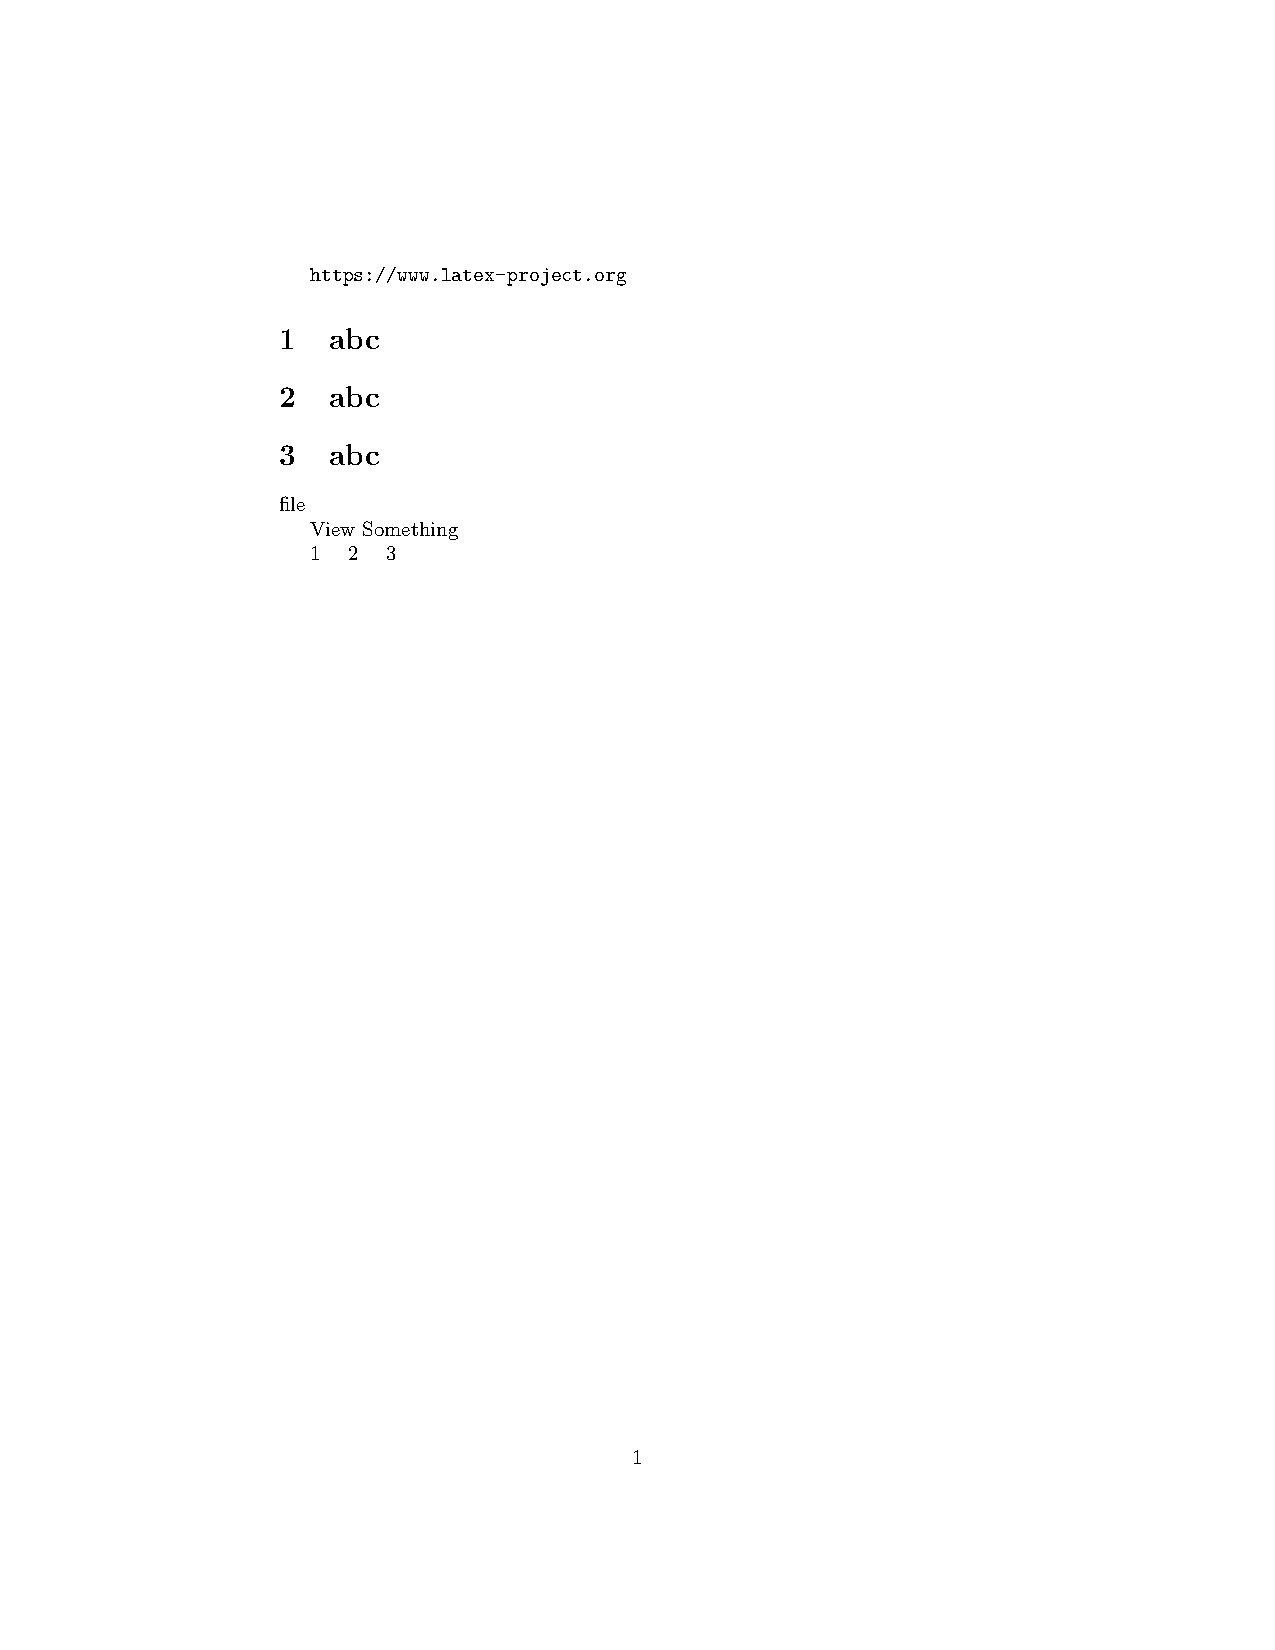
\includepdf[pages=-]{pax-input}
\fbox{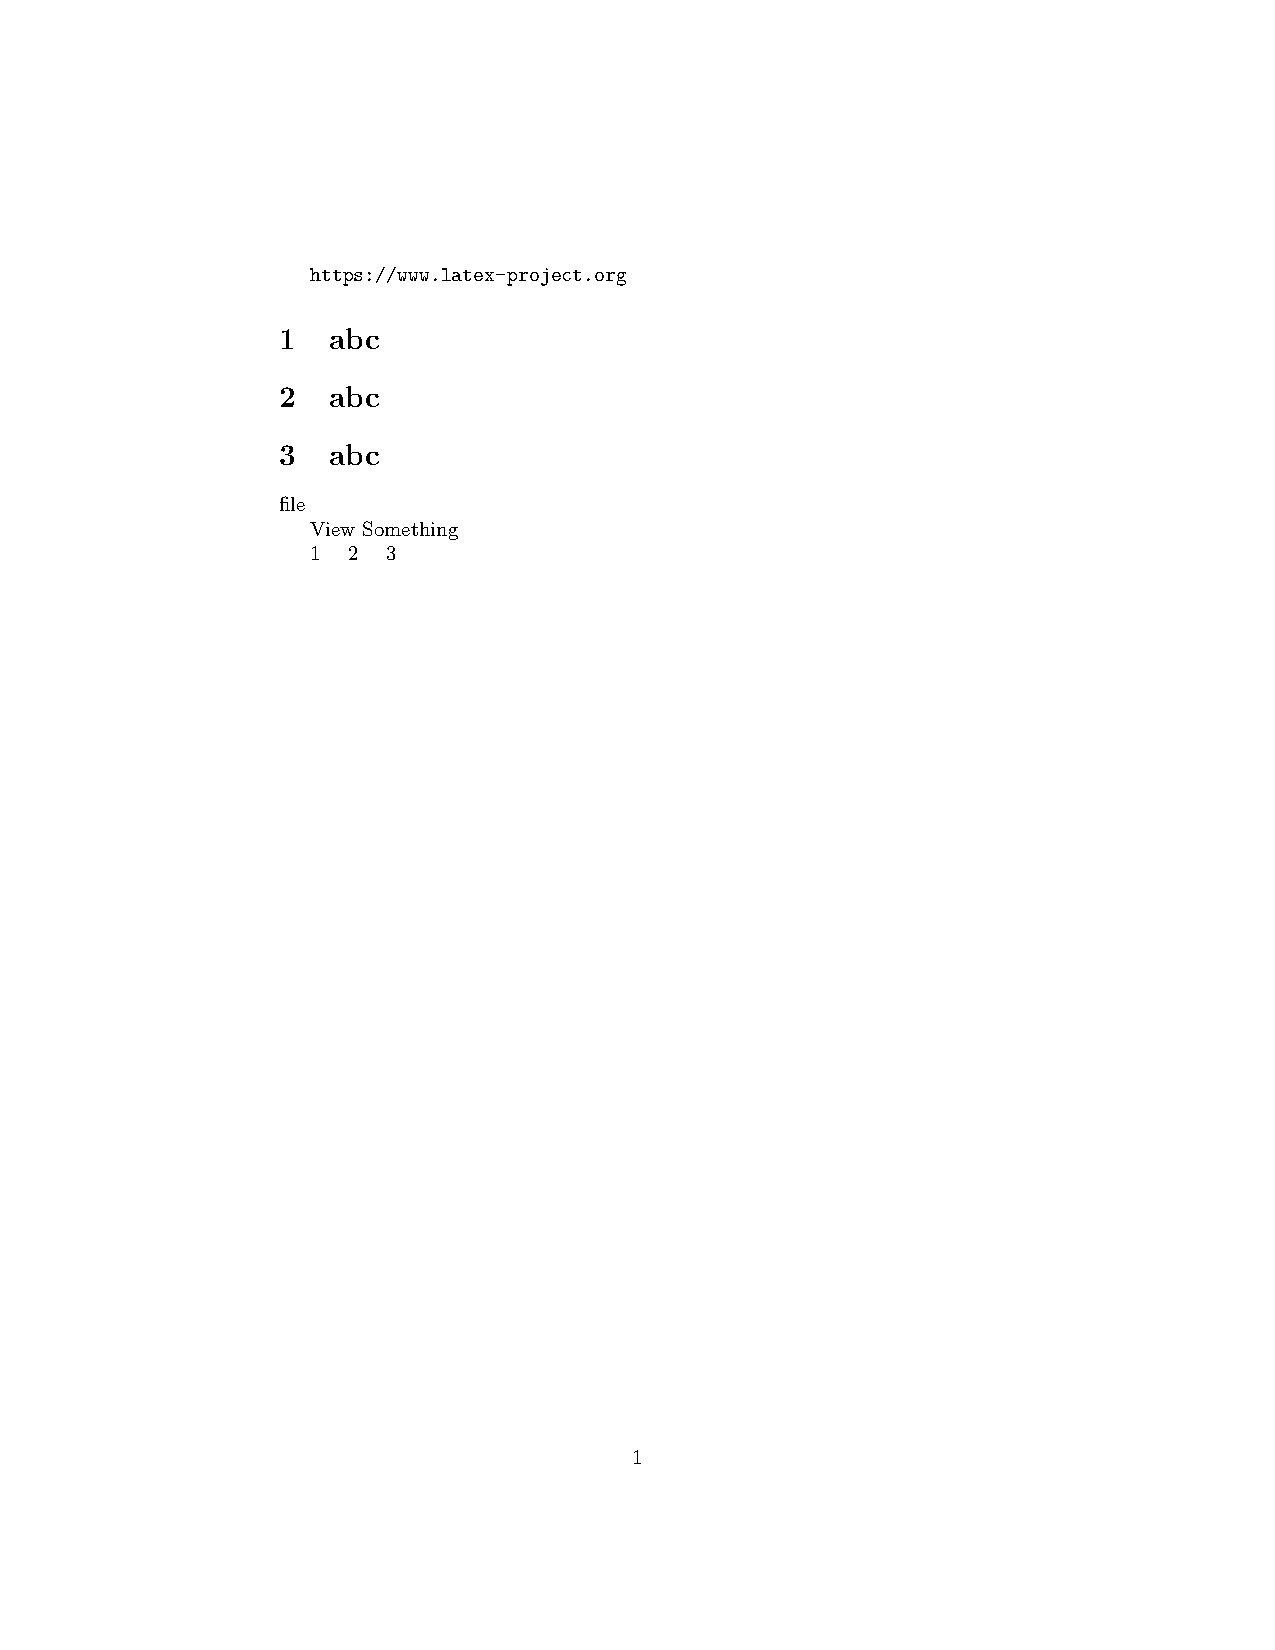
\includegraphics[scale=0.5]{pax-input}}

\makeatletter \def\blb{abc düß}
%\@PAX@escapename@NV \blub \blb
%\show\blub
\ExplSyntaxOn
\ExplSyntaxOff

%\includegraphics[page=2]{pax-input}
%\insertlink blbbl
bkbkb
%\includepdf[pagecommand={\insertlink}]{testinput}
\end{document}
\usepackage{pax} 